\documentclass[dvipdfmx, 9pt, a4paper]{jsarticle}
\usepackage[margin=15mm]{geometry}
\usepackage{fancyhdr}
\usepackage{multirow}
\usepackage{amsmath,  amssymb}
\usepackage{type1cm}
\usepackage{latexsym}
\usepackage{algorithmic}
\usepackage{algorithm}
\usepackage{ascmac}
\usepackage{braket}
\usepackage{listings,jvlisting}
\usepackage{tcolorbox}
\usepackage[utf8]{inputenc}
\usepackage{color}

\renewcommand{\theequation}{\arabic{section}.\arabic{equation}}
\renewcommand{\thefigure}{\arabic{section}.\arabic{figure}}
\renewcommand{\thetable}{\arabic{section}.\arabic{table}}
\makeatletter
\@addtoreset{equation}{section}
\@addtoreset{figure}{section}
\@addtoreset{table}{section}
\AtBeginDocument{
  \renewcommand*{\thelstlisting}{\arabic{section}.\arabic{lstlisting}}%
  \@addtoreset{lstlisting}{section}
}


\numberwithin{equation}{section}

\DeclareFixedFont{\ttb}{T1}{txtt}{bx}{n}{9}
\DeclareFixedFont{\ttm}{T1}{txtt}{m}{n}{9}
\definecolor{deepblue}{rgb}{0,0,0.5}
\definecolor{deepred}{rgb}{0.6,0,0}
\definecolor{deepgreen}{rgb}{0,0.5,0}

\renewcommand{\baselinestretch}{0.78}
\newcommand{\bm}[1]{{\mbox{\boldmath $#1$}}}
\newcommand{\bnabla}{\bm \nabla}
\newtheorem{Proof}{証明}
\def\qed{\hfill $\Box$}

\newcommand\pythonstyle{\lstset{
language=Python,
basicstyle=\ttm,
morekeywords={self},
keywordstyle=\ttb\color{deepblue},
emph={MyClass,__init__},
emphstyle=\ttb\color{deepred},
stringstyle=\color{deepgreen},
frame=tb,
showstringspaces=false
}}

\lstnewenvironment{python}[1][]
{
\pythonstyle
\lstset{#1}
}
{}

\newcommand\pythonexternal[2][]{{
\pythonstyle
\lstinputlisting[#1]{#2}}}
\newcommand\pythoninline[1]{{\pythonstyle\lstinline!#1!}}

\begin{document}
\begin{center}
{\fontsize{18pt}{1pt}\selectfont 有限要素法}\\
\end{center}
\section*{はじめに}
エンジニアリングにおいて重要な物理現象の多くは偏微分方程式で表現できるが、任意の境界条件(B.C.)や初期条件(I.C.)に対する偏微分方程式の解を解析的に解くことは不可能である。それゆえ数値計算による近似解法が必要になってくる訳だが、有限要素法(FEM)は数ある手法の中でも最も有名だろう。\par
FEMは格子法に分類される手法であり、解析対象の領域をメッシュで離散化する。メッシュには節点と複数の節点で構成される要素の情報が含まれる。数値計算においてはFDMと同様に、節点上の物理場の値のみ明示的に考える。しかしながらFDMと異なり、節点以外の点に関しては多項式などで補間する。つまり、FEMは節点上の物理量を明示的に考えつつその値から導かれる補間関数を要素毎に定めることで、系全体の近似関数を求めている。\par
補間関数を求める上で重要となるのが形状関数である。補間関数は節点における物理量にも依存するのに対し、形状関数はメッシュ形状にのみ依存する。形状関数を用いることで、補間関数の導出が容易になる。\par
また、FEMでは支配方程式の弱形式と呼ばれるものを利用する。後述するようにFDMなどでは強形式を用いる訳であるが、それをわざわざ弱形式に変換する理由として、近似関数の滑らかさに関する条件の緩和や計算効率性などが挙げられる。しかしながら、この弱形式のややこしさがFEMを他の手法よりも難解なものにしているのかもしれない。\par
そこで本資料ではFEMの難解さを鑑みて、いきなりFEM全般を議論するのではなく、簡単な物理現象から具体的な議論を始めて、最終的にFEM全般が理解できるような進め方にした。1章では物理問題と無関係な形状関数について議論する。2章から物理問題の求解について議論していき、章が進む毎に複雑と思える問題に取り組むことにした。

\section{形状関数}
本章ではFEMの近似処理を担う形状関数について議論する。先述の通りFEMは領域をメッシュで分割し、各要素の物理場を多項式で補間する。要素間の物理量は一般的に連続でなければならないので、多項式の値も節点および要素境界上で一致しなければならない。このような補間関数は節点における物理量及び形状関数から求められる。
\subsection{1次元空間における形状関数}
まずは1次元空間における形状関数について考える。先述の通りメッシュの要素は節点により構成されるが、要素当たりの節点の数は任意である。1次元空間ならば、要素に対する節点数として2つ(両端が節点)の場合を想像するかもしれないが、実は中間部分に節点があってもよい(図1)。そしてFEMでは節点上の物理量が所与のものであると考えて、要素内を近似関数で補間する。\par
\begin{figure}[b]
\begin{center}
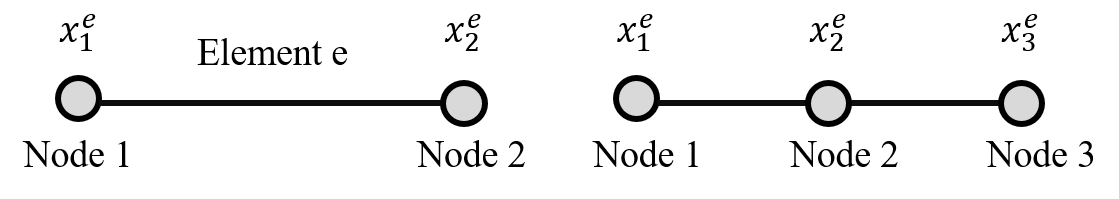
\includegraphics[width = 10cm]{fig1_1.png}
\caption{1次元空間における要素と節点分布の例。}
\end{center}
\end{figure}
例えば近似関数が多項式である場合、物理量$\theta^e$は
\begin{equation}
\theta^e(x)=\alpha^e_0 + \alpha^e_1x + \alpha^e_2 x^2 + ... + \alpha^e_mx^m = 
\begin{bmatrix}
1 & x & x^2 & ... x^m
\end{bmatrix}
\begin{bmatrix}
\alpha^e_0 \\ \alpha^e_1 \\ ... \\ \alpha^e_m
\end{bmatrix}=\bm p^{\rm T}(x)\bm \alpha^e
\end{equation}
のように書き表される。ここで$x$は位置座標、$\alpha_i$は係数である。また上付き文字$e$は要素毎に定義されるものであることを示している。\par
係数は節点上の物理量$\theta^e(x^e_i) = \theta^e_i$より求める。従って、節点数が$n$の場合、$(n-1)$次の多項式で近似することができる。このとき、
\begin{equation}
\bm \theta^e = 
\begin{bmatrix}
\theta^e_1 \\ \theta^e_2 \\ ... \\ \theta^e_n
\end{bmatrix}=
\begin{bmatrix}
1 & x^e_1 & x^{e2}_1 & ... & x^{e(n-1)}_1 \\
1 & x^e_2 & x^{e2}_2 & ... & x^{e(n-1)}_2 \\
... & ... & ... & ... & ... \\
1 & x^e_n & x^{e2}_n & ... & x^{e(n-1)}_n \\
\end{bmatrix}
\begin{bmatrix}
\alpha^e_0 \\ \alpha^e_1 \\ ... \\ \alpha^e_n
\end{bmatrix}
=M^e\bm \alpha^e \notag
\end{equation}
より、$\alpha = M^{e(-1)}\bm \theta$だと分かる。従って式(1.1)より
\begin{equation}
\theta^e(x)=\bm p^{\rm T}(x)M^{e(-1)}\bm \theta^e \notag
\end{equation}
と多項式が求まる。ここで$N^e(x)=\bm p^{\rm T}(x)M^{e(-1)} \in \mathbb{R}^{1 \times n}$のことを形状関数行列、各項のことを形状関数と言う。形状関数を用いることで、要素内の分布は
\begin{equation}
\theta^e(x)=N^e(x)\bm \theta^e = \sum N^e_i(x)\theta^e_i
\end{equation}
と求まる。証明は省くが、1次元要素形状関数について以下の定理が知られている。
\begin{itembox}[l]{定理1.1}
 1次元要素形状関数はクロネッカー・デルタの性質を有する。つまり$N^e_i(x^e_j)=\delta_{ij}$である。
\end{itembox}
\subsubsection{2節点1次要素における形状関数}
形状関数の最も単純な例として、図1左に示すような2節点1次要素の問題を考える。要素当たり2つの節点しかないため、補間関数には1次関数$\alpha^e_0+\alpha^e_1x$が利用できる。多項式の係数を決定する上で節点位置は任意だが、一般的には要素の両端に節点があるとする。この場合、定理1.1より形状関数は以下のように書き表される。
\begin{equation}
N^e(x)=
\begin{bmatrix}
N^e_1(x) & N^e_2(x)
\end{bmatrix}
=\frac{1}{l^e}
\begin{bmatrix}
x^e_2 - x & x - x^e_1
\end{bmatrix},~~~l^e = x^e_2 - x^e_1
\end{equation}\par
後述するように、FEMでは物理量の勾配をよく計算する。これは支配方程式中に物理量の勾配がよく登場することから容易に想像できるであろう。式(1.2)より、$\theta^e(x)$の勾配は形状関数行列の微分$B^e=(\partial_xN^e_1(x), \partial_xN^e_2(x), ....) \in \mathbb{R}^{1\times n}$を用いて
\begin{equation}
\partial_x\theta^e(x)=B^e\bm \theta^e
\end{equation}
と書き表される。このような行列$B^e$をBマトリックスと言う。2節点1次要素におけるBマトリックスを以下に示す。
\begin{equation}
B^e = \frac{1}{l^e}
\begin{bmatrix}
-1 & 1
\end{bmatrix}
\end{equation}
\subsubsection{1次元2次要素における形状関数}
次に2次の多項式で分布を補間することを考える。この場合係数の数は3つなので、図1右のように要素は3つの節点で構成されていなければならない。節点位置は任意だが、両端に2つと中央に1つ設けることが多い。式(1.2)より多項式$\theta^e(x)$が2次であるならば、対応する形状関数も2次の多項式であり、形状関数関数行列は$(N^e_1(x), N^e_2(x), N^e_3(x))$となる。任意の2次多項式は
\begin{equation}
N^e_i(x)=\frac{(x-a)(x-b)}{c} \notag
\end{equation}
のように書き表される(ただし$c \neq 0$)。定理1.1の条件より各$N^e_i(x)$の未知数$a$、$b$、$c$は定まり、以下のように求まる。
\begin{equation}
N^e_1(x)=\frac{(x-x_2^e)(x-x_3^e)}{(x_1-x_2^e)(x_1-x_3^e)},~~~N^e_2(x)=\frac{(x-x_1^e)(x-x_3^e)}{(x_2-x_1^e)(x_2-x_3^e)},~~~N^e_3(x)=\frac{(x-x_1^e)(x-x_2^e)}{(x_3-x_1^e)(x_3-x_2^e)}
\end{equation}

\subsection{1次元空間におけるガウス積分}
後述するようにFEMでは物理量の分布関数$\theta(x)$(式(1.2))の積分を求めなければならない。積分値の数値計算手法として矩形積分や台形積分が有名だが、対象の関数が多項式である場合、ガウス積分を用いることができる。\par
本節では一般的な議論を展開するために、$I=\int_a^b f(x) {\rm d}x$を考えることにする。まず初めに、積分区間$[a, b]$は任意であるがガウス積分では$[-1, 1]$として定式化している。したがって最初に変数$x$の線形変換をしなければならない。$x$を$\xi$に変換するとしたとき、両者の関係は
\begin{equation}
x = \frac{1}{2}(a+b) + \frac{1}{2}\xi(b-a) \notag
\end{equation}
となる。従って積分値は
\begin{equation}
I=\frac{b-a}{2}\int_{-1}^1f(\xi){\rm d}\xi=J\hat{I}
\end{equation}
のように書き表される。ガウス積分は上式の$\hat{I}$を求める術を教えてくれる。
\begin{tcolorbox}[title=1次元空間におけるガウス積分]
 $p$次の多項式$f(\xi)$の積分$\hat{I}=\int_{-1}^1f(\xi) {\rm d}x$を考える。$n_{gp}$を$n_{gp} \geq (p+1)/2$を満たす最小の整数とする。このとき、表1.1の積分点$\xi_i$と重み$W_i$を用いて、積分を以下の式より求める。
\begin{equation}
\hat{I}=\sum W_if(\xi_i)
\end{equation}
\end{tcolorbox}

\begin{table}[t]
\begin{center}
\caption{1次元空間におけるガウス積分の積分点と重み}
\begin{tabular}{ccc}
\hline \hline
$n_{gp}$ & $\xi_i$ & $W_i$ \\ \hline \hline
1 & 0.0 & 2.0 \\ \hline
2 & $\pm 1/\sqrt{3}$ & 1.0 \\ \hline
3 & $\pm0.7745966692$ & 0.5555555556 \\
 & 00 & 0.8888888889 \\ \hline
4 & $\pm 0.8611363116$ & 0.3478548451 \\
 & $\pm 0.3399810436$ & 0.3478548451 \\ \hline
\end{tabular}
\end{center}
\end{table}

\subsection{2次元空間における形状関数}
本節では2次元空間における形状関数について考える。実は2次元になった途端に形状関数の数学的議論は1次元空間のときから非常に難しくなる。例えば図1.2のような隣接する2要素を考えよう。この場合も1次元空間のときと同様で、各要素に多項関数$\theta^e(x, y)$を設定する。系全体の状態はこれら多項関数の和で表現される訳だが、場の関数が連続であることを鑑みたとき、要素1の多項関数$\theta^1(x, y)$と要素2の多項関数$\theta^2(x,y)$は辺$ac$上の点で同じ値とならなければならない。\par
1次元空間の場合、図1.1のように要素の端部に節点を設けたならばこのような心配はする必要がなかった。補間関数が節点上で所与の値になるように定められてさえいれば、自ずと連続性が満たされるためである。一方で2次元空間の場合、点$a$と$c$で両関数が同じ値となっただけでは連続性は保証されない。\par
関数の連続性は多項関数の完全性と絡めることで議論されている。しかしながら本資料ではそこまで踏み込まないことにし、代表的な形状における形状関数を紹介するだけに留める。まず、4節点長方形要素における形状関数を議論する。この形状関数はアイソパラメトリック要素という手法を用いることで長方形以外の四角形要素でも利用可能になる。次にアイソパラメトリック要素の概念を適用して3節点三角形要素に対する形状関数を議論する。1.1節では2次多項関数の形状関数も紹介したが、本節では話を簡単にするため線形な形状関数のみ考える。また、節点は四角形および三角形の頂点に位置するものと考える。

\begin{figure}[t]
\begin{center}
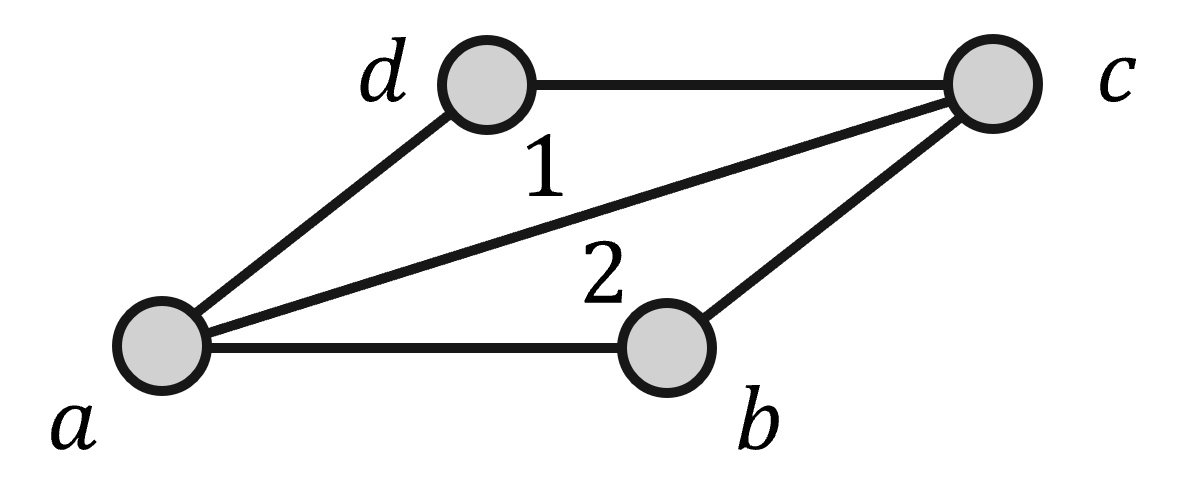
\includegraphics[width = 5cm]{fig1_2.png}
\caption{2次元空間における要素と節点分布の例。}
\end{center}
\end{figure}

\subsubsection{4節点長方形要素}
\begin{figure}[b]
\begin{center}
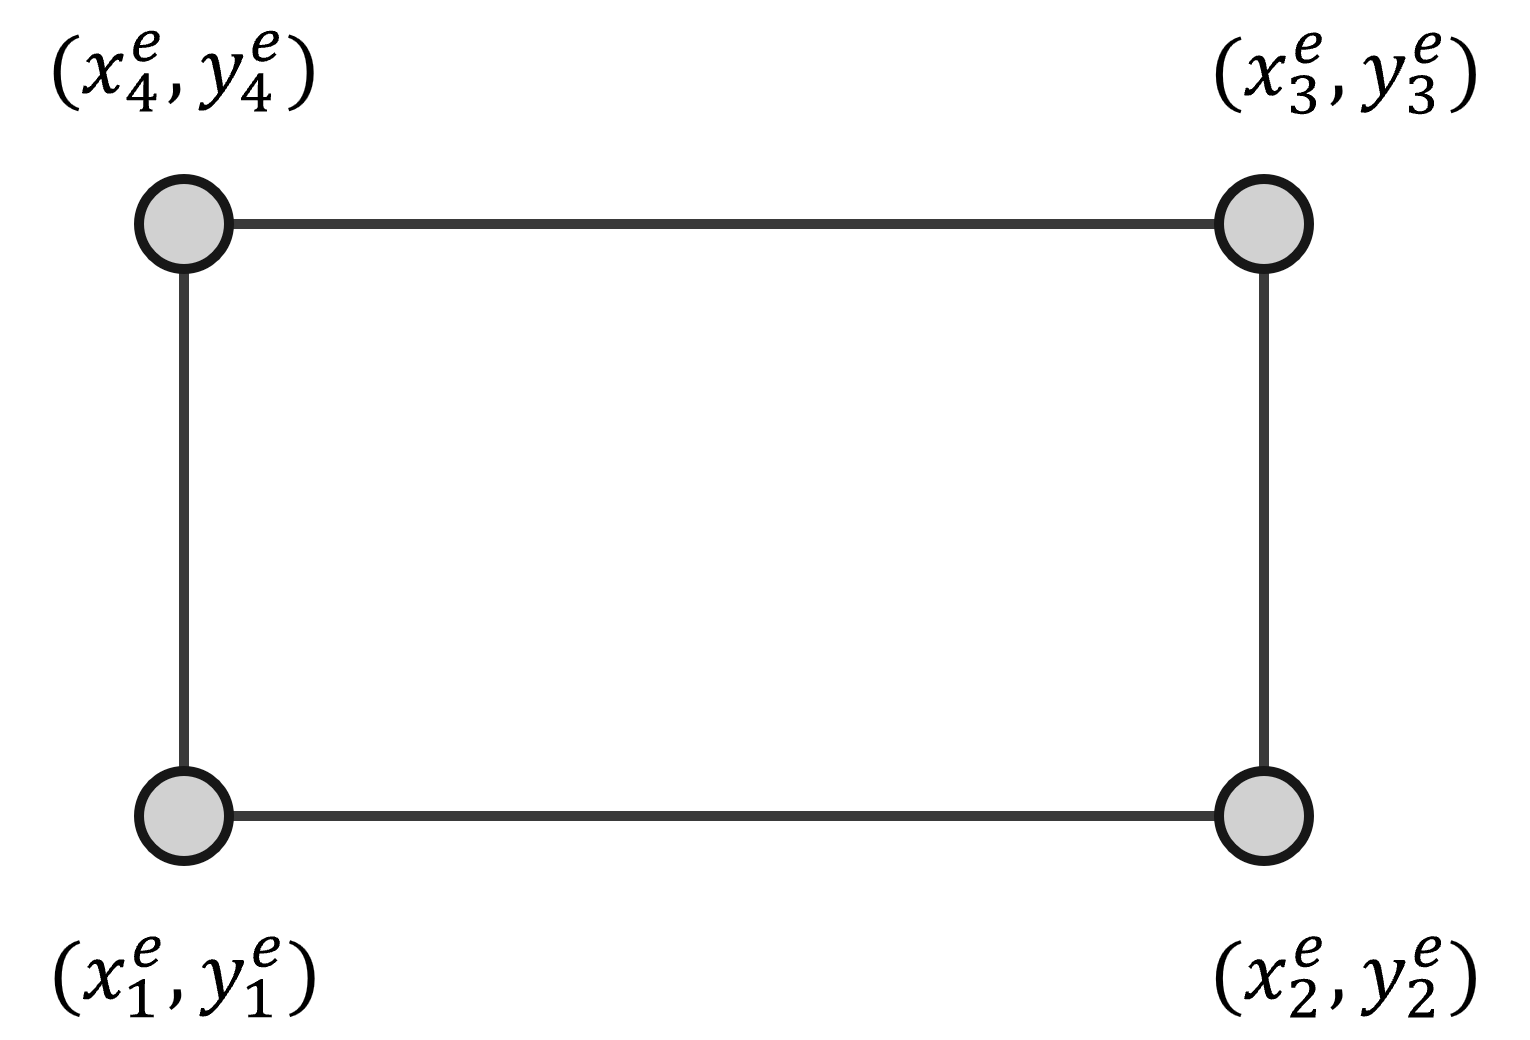
\includegraphics[width = 5cm]{fig1_4.png}
\caption{4節点長方形要素}
\end{center}
\end{figure}

図1.3のような4節点長方形要素における形状関数を考える(本項で紹介する形状関数は任意の四角形に適用可能なものでないことに注意)。この場合、補間関数に$\theta^e(x, y)=\alpha^e_0 + \alpha^e_1x+\alpha^e_2y+\alpha^e_3xy$を用いればよい。頂点上の物理量$\theta^e_i$は所与であると考えるため、4つの多項式が得られる。従って1.1節と同様に連立一次方程式から形状関数を導出することができる。ここでは導出を省き、結果のみ示す。
\begin{equation}
\begin{array}{l}
N^e_1(x,y)=(x-x^e_2)(y-y^e_4)/A^e \\
N^e_2(x,y)=-(x-x^e_1)(y-y^e_4)/A^e \\
N^e_3(x,y)=(x-x^e_1)(y-y^e_1)/A^e \\
N^e_4(x,y)=-(x-x^e_2)(y-y^e_1)/A^e \\
\end{array}
\end{equation}
ここで$A^e$は長方形の面積である。\par
このような解き方はもちろん正しいが、より簡単に計算できる方法がある。実は長方形要素に対する2次元形状関数は1次元の形状関数の積により得られる。例えば形状関数$N^e_2(x, y)$は点$(x^e_2, y^e_2)$で1、その他の頂点で0となればよいので、$N^e_2(x, y)=N^e_2(x)N^e_1(y)$となる。ここで$N^e_2(x)$は領域$(x^e_1, x^e_2)$における1次元形状関数(式(1.3))であり、$N^e_1(y)$は領域$(y^e_1, y^e_4)$における1次元形状関数(式(1.3))である。以上より、2次元に対する形状関数は以下のようにも表現できる。
\begin{equation}
N^e_1(x, y)=N^e_1(x)N^e_1(y),~~~N^e_2(x, y)=N^e_2(x)N^e_1(y),~~~N^e_3(x, y)=N^e_2(x)N^e_2(y),~~~N^e_4(x, y)=N^e_1(x)N^e_2(y)
\end{equation}\par
最後にBマトリックスを考えていく。定義より$\theta^e(x, y)=N^e\bm \theta^e$であるため、
\begin{equation}
\bnabla \theta=
\begin{bmatrix}
\partial_x \theta^e \\ \partial_y \theta^e
\end{bmatrix}=
\begin{bmatrix}
\partial_x N^e_1 & \partial_x N^e_2 & \partial_x N^e_3 & \partial_x N^e_4 \\
\partial_y N^e_1 & \partial_y N^e_2 & \partial_y N^e_3 & \partial_y N^e_4
\end{bmatrix}\bm \theta^e \notag
\end{equation}
なる関係が得られる。従ってBマトリックスは2行4列の行列であり、以下のように書き表される。
\begin{equation}
B^e=\frac{1}{A^e}
\begin{bmatrix}
y-y^e_4 & -y+y^e_4 & y-y^e_1 & -y+y^e_1 \\
x-x^e_2 & -x+x^e_1 & x-x^e_1 & -x+x^e_2
\end{bmatrix}
\end{equation}

\subsubsection{4節点四角形要素}
\begin{figure}[t]
\begin{center}
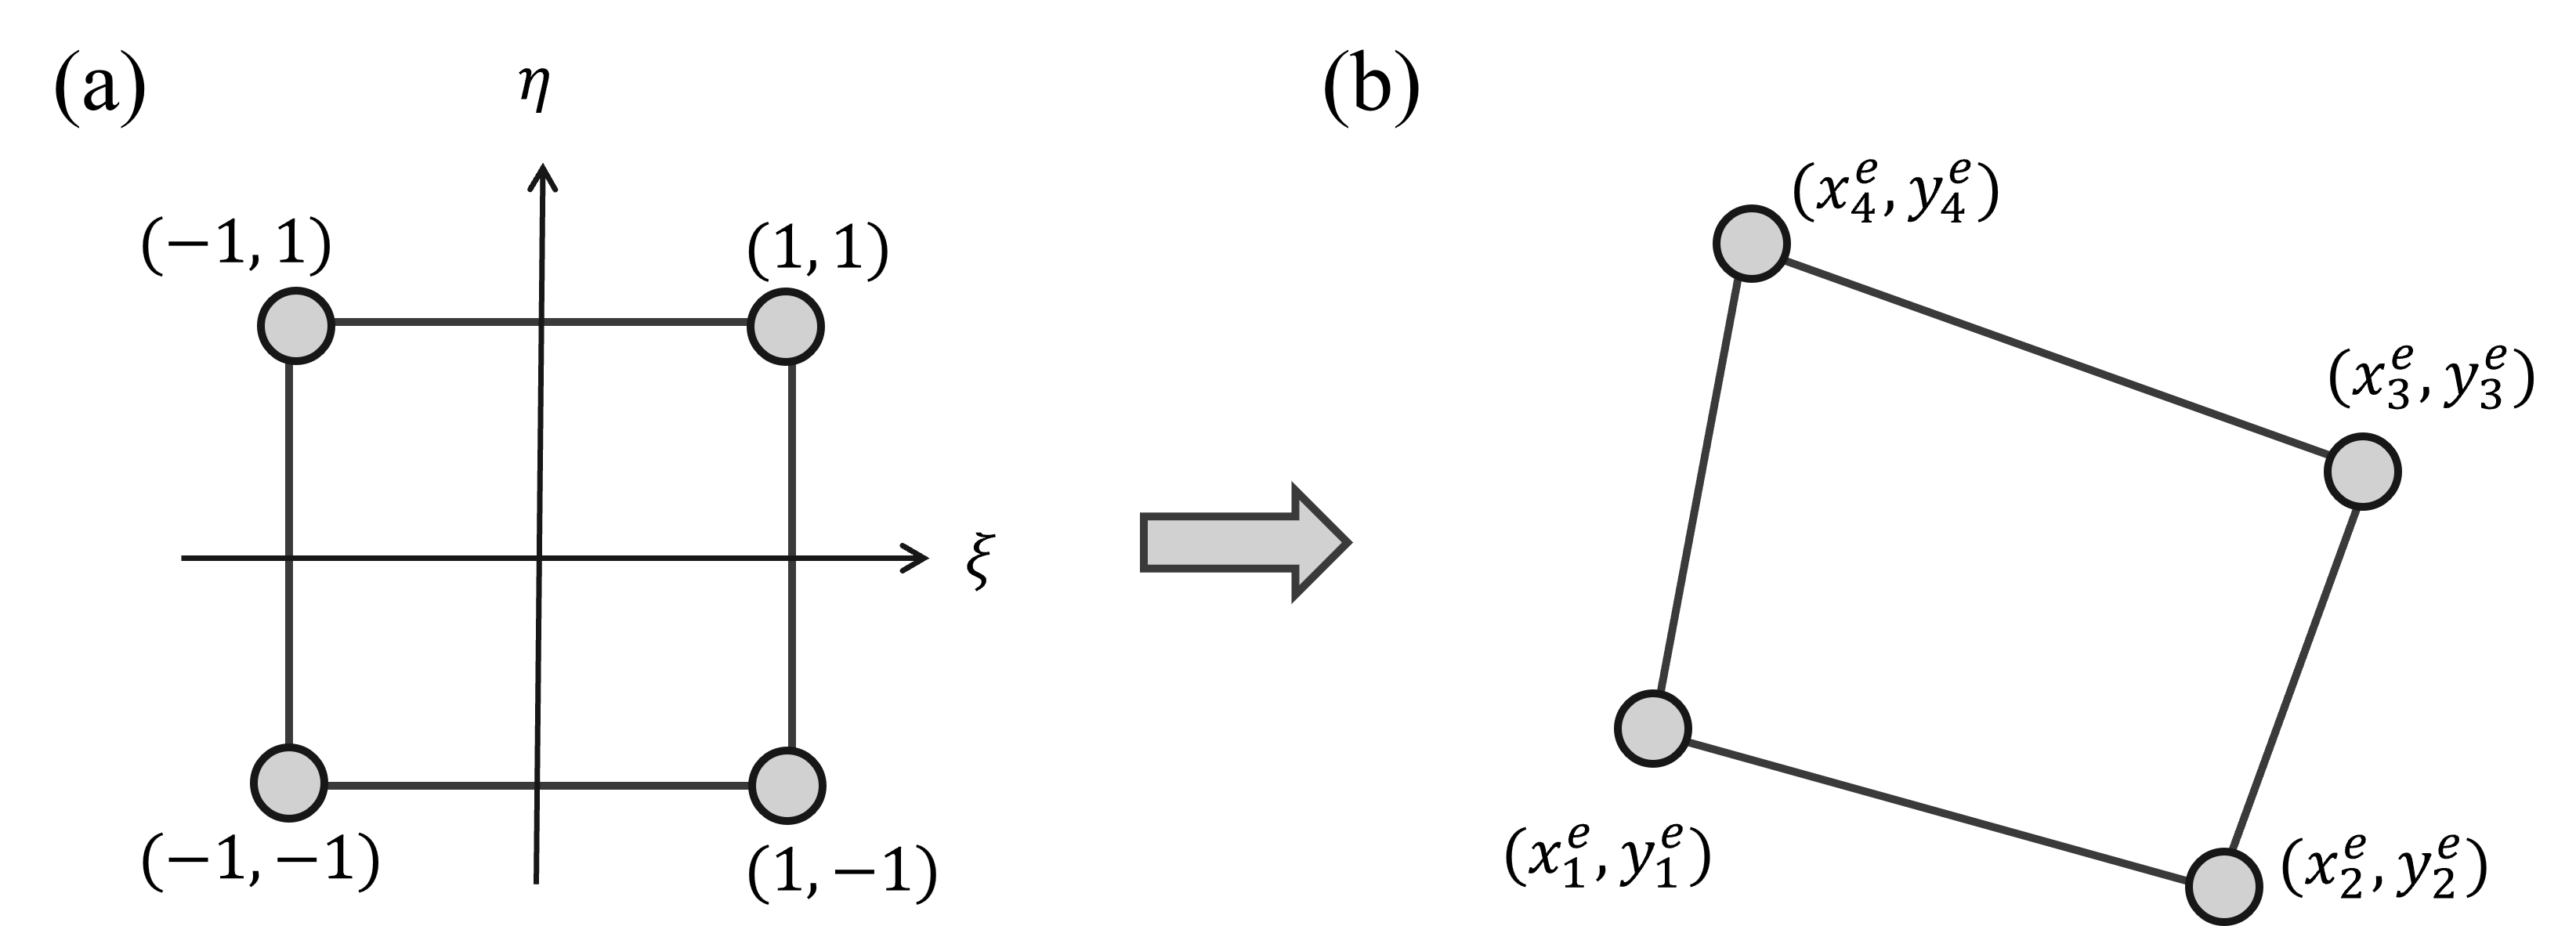
\includegraphics[width = 10cm]{fig1_5.png}
\caption{4節点4角形要素(a)親座標(b)物理座標}
\end{center}
\end{figure}

本項では図1.4(b)のような4節点四角形要素における形状関数について議論する。説明はしなかったが、長方形でない四角形に対して補間関数$\theta^e(x, y)=\alpha^e_0 + \alpha^e_1x+\alpha^e_2y+\alpha^e_3xy$は連続性を満たさない。そのため別の形状関数が必要となる訳だが、ここではアイソパラメトリック要素という手法を紹介する。\par
まず、図1.4(a)に示すような$\xi-\eta$の座標系と、各軸$[-1,1]$の領域の正方形を考える。このような座標系を親座標、領域$[-1,1]$を親領域と言う。一方の図1.4(b)の座標を物理座標、領域を物理領域と言う。いま図1.4(b)の四角形は図1.4(a)の四角形から変換されたものとして考えよう。両図の各頂点が対応するような変換を考えたとき、つまり例えば$(\xi, \eta)=(-1, -1)$の点の写像結果の$x$は$x^e_1$であるように考えたとき、この変換は式(1.9)の形状関数を用いて表現できる。
\begin{equation}
x(\xi, \eta) = N
\begin{bmatrix}
x^e_1 \\ x^e_2 \\ x^e_3 \\ x^e_4
\end{bmatrix}=N(\xi, \eta)\bm x^e,~~~
y(\xi, \eta) = N
\begin{bmatrix}
y^e_1 \\ y^e_2 \\ y^e_3 \\ y^e_4
\end{bmatrix}=N(\xi, \eta)\bm y^e,~~~
N=\begin{bmatrix}
N_1(\xi, \eta), N_2(\xi, \eta), N_3(\xi, \eta), N_4(\xi, \eta)
\end{bmatrix}
\end{equation}
なお、図1.4(a)の親領域における形状関数は
\begin{equation}
N_i(\xi, \eta)=\frac{1}{4}(1+\xi_i\xi)(1+\eta_i\eta)
\end{equation}
のようにシンプルに書き表すことができる(親領域には常に図1.4(a)のようなものを使う。従って形状関数に上付き文字の$e$を付けなくても誤解を招かない)。ここで$\eta_i$と$\xi_i$の値は表1.2の通りである。\par
\begin{table}[b]
\begin{center}
\caption{式(1.13)中の係数値一覧}
\begin{tabular}{c|cccc}
\hline
node number & 1 & 2 & 3 & 4 \\ \hline
$\xi_i$ & -1 & 1 & 1 & -1 \\
$\eta_i$ & -1 & -1 & 1 & 1 \\ \hline
\end{tabular}
\end{center}
\end{table}
前項で説明しなかったが、式(1.9)の形状関数ならば写像の線形性が満たされる。つまり例えば$(\xi, \eta)$が(-1, -1)と(1, -1)の間の任意の点は$(x, y)$が$(x^e_1, y^e_1)$と$(x^e_2, y^e_2)$の間の点に写像される。親領域の写像によって得られる物理領域も基本的に四角形となる。\par
物理量の補間関数についても親座標で考える。このとき、$(\xi, \eta)$における物理量は式(1.9)の形状関数を用いて
\begin{equation}
\theta^e(\xi, \eta)=
\begin{bmatrix}
N_1(\xi, \eta) & N_2(\xi, \eta) & N_3(\xi, \eta) & N_4(\xi, \eta)
\end{bmatrix}
\begin{bmatrix}
\theta^e_1 \\ \theta^e_2 \\ \theta^e_3 \\ \theta^e_4
\end{bmatrix}=N\bm \theta^e
\end{equation}
のように書き表すことができる。ここで各$\theta^e_i$は物理領域の頂点における物理量である。式(1.12)より親座標と物理座標の各点は一対一に対応しているので、$\theta^e(\xi, \eta)$から$\theta^e(x, y)$を求めることは可能である。また、次節で紹介する多次元のガウス積分を用いることで、$\theta^e(x, y)$の空間積分も$\theta^e(\xi, \eta)$から求めることができる。\par
$\theta^e(x, y)$の勾配も$\theta^e(\xi, \eta)$の結果から求めることができる。まず、本来知りたかった物理座標に対する未知の形状関数を$N^{e*}_i(x, y)$と置く。このとき、$\theta^e(x, y)$は$\theta^e(x, y)=N^{e*}(x, y)\bm \theta$のように書き表すことができる。この形状関数行列に対するBマトリックスは
\begin{equation}
B^e=
\begin{bmatrix}
\partial_xN^{e*}_1(x, y) & \partial_xN^{e*}_2(x, y)& \partial_xN^{e*}_3(x, y) & \partial_xN^{e*}_4(x, y) \\
\partial_yN^{e*}_1(x, y) & \partial_yN^{e*}_2(x, y) & \partial_yN^{e*}_3(x, y) & \partial_yN^{e*}_4(x, y) \\
\end{bmatrix} \notag
\end{equation}
である。連鎖率より$N^{e*}_i(x, y)$の親座標に対する微分は
\begin{equation}
\begin{bmatrix}
\partial_\xi N^{e*}_i(x, y) \\ \partial_\eta N^{e*}_i(x, y)
\end{bmatrix}=
\begin{bmatrix}
\partial_\xi x & \partial_\xi y \\
\partial_\eta x & \partial_\eta y \\
\end{bmatrix}
\begin{bmatrix}
\partial_x N^{e*}_i(x, y) \\ \partial_y N^{e*}_i(x, y)
\end{bmatrix}
=J^e
\begin{bmatrix}
\partial_x N^{e*}_i(x, y) \\ \partial_y N^{e*}_i(x, y)
\end{bmatrix} \notag
\end{equation}
となる。ここで$J^e$は物理座標を親座標で微分したときのヤコビ行列である。$J^e$が正則であるならば、所望の微分は
\begin{equation}
\begin{bmatrix}
\partial_x N^{e*}_i(x, y) \\ \partial_y N^{e*}_i(x, y)
\end{bmatrix}=J^{^e(-1)}
\begin{bmatrix}
\partial_\xi N^{e*}_i(x, y) \\ \partial_\eta N^{e*}_i(x, y)
\end{bmatrix}=J^{e(-1)}GN^{e*}_i(x, y),~~~G=
\begin{bmatrix}
\partial_\xi \\ \partial_\eta
\end{bmatrix}
\end{equation}
より求まる。$J^e$について式(1.12)を代入すると
\begin{equation}
J=GN(\xi, \eta)
\begin{bmatrix}
\bm x^e & \bm y^e
\end{bmatrix},~~~N=\begin{bmatrix}
N_1(\xi, \eta), N_2(\xi, \eta), N_3(\xi, \eta), N_4(\xi, \eta)
\end{bmatrix} \notag
\end{equation}
であることが分かるため、以上より所望のBマトリックスは
\begin{equation}
B=J^{e(-1)}GN
\end{equation}
と求まる。このようにBマトリックスはヤコビ行列の逆行列と親座標に関する形状関数から計算できる。\par
最後に、ヤコビ行列は当然ながら正則でなければならないことを改めて注記しておく。また、加えてヤコビ行列の行列式は非ゼロでなければならない。この条件は、図1.4(b)の四角形に$\pi$以上の内角が無いときに満たされる。

\subsubsection{3節点三角形要素}
\begin{figure}[b]
\begin{center}
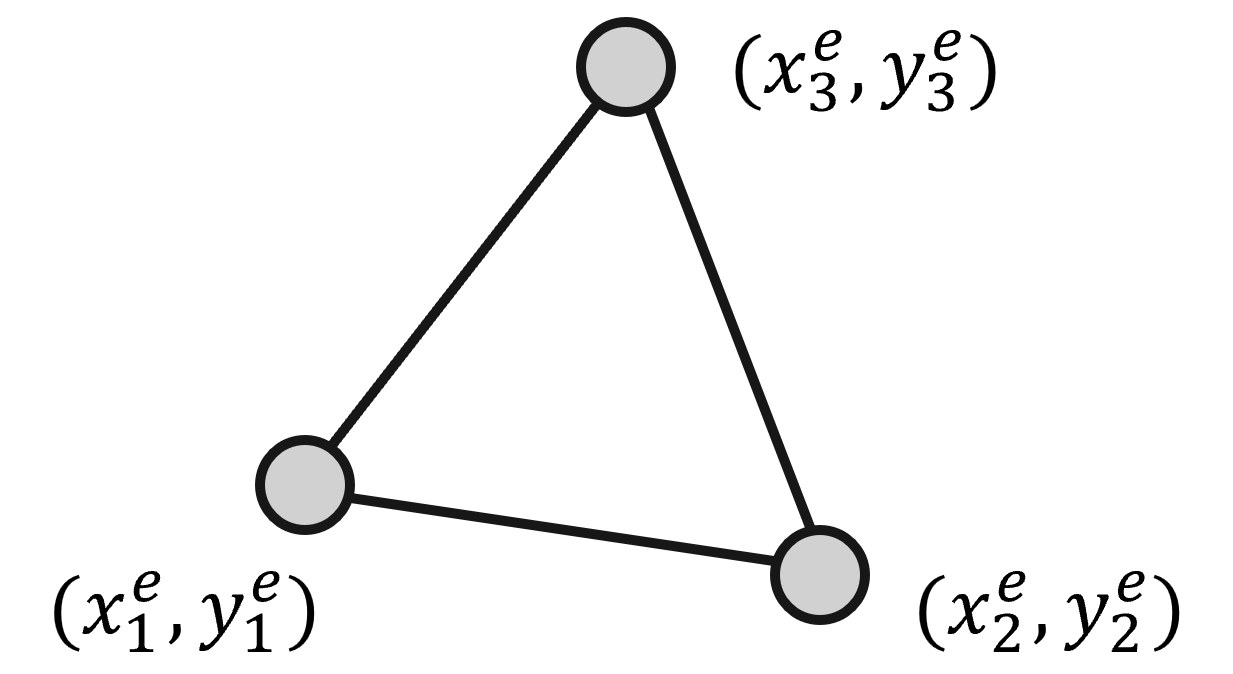
\includegraphics[width = 5cm]{fig1_3.png}
\caption{3節点三角形要素}
\end{center}
\end{figure}

本節の最後に3節点三角形要素に対する形状関数を議論する。これも1.1節と同様に連立一次方程式から計算できるが、ここでは面積座標による表現を紹介する。\par
まず図1.6(a)のように任意の点$P$を用いて図1.5の三角形を3つに分割する。それぞれの面積を$A_i(i=1,2,3)$としたとき、変数$\xi_i$を
\begin{equation}
\xi_i=\frac{A_i}{A}
\end{equation}
と定義する。ここで$A=\sum_iA_i$であり、図1.5の頂点を用いて
\begin{equation}
A=(x^e_2y^e_3-x^e_3y^e_2)-(x^e_1y^e_3-x^e_3y^e_1)+(x^e_1y^e_2-x^e_2y^e_1)
\end{equation}
のように書き表される。変数の組$(\xi_1, \xi_2, \xi_3)$のことを面積座標と言う。定義より$\xi_i$には
\begin{equation}
\xi_1+\xi_2+\xi_3=1
\end{equation}
なる関係式が存在するため、面積座標の次元は2であることが分かる。また、明らかに面積座標と物理座標$(x, y)$には一対一の関係がある。\par
各面積$A_i$は式(1.18)と同様の式で求められることを考えると、物理座標と面積座標の間には線形関係が成り立つことが分かる。加えて$P$が頂点$i$であるとき$\xi_j=\delta_{ij}$であることを考えると、物理座標は
\begin{equation}
x=\sum x^e_i \xi_i,~~~y=\sum y^e_i\xi_i
\end{equation}
のように書き表せると分かる。式(1.19)(1.20)より
\begin{equation}
\begin{bmatrix}
1 & x & y
\end{bmatrix}=
\begin{bmatrix}
1 & 1 & 1 \\
x^e_1 & x^e_2 & x^e_3 \\
y^e_1 & y^e_2 & y^e_3
\end{bmatrix}
\begin{bmatrix}
\xi_1 \\ \xi_2 \\ \xi_3
\end{bmatrix} \notag
\end{equation}
の関係が言えるため、物理座標から面積座標に変換したい場合は逆行列を求めて
\begin{equation}
\begin{bmatrix}
\xi_1 \\ \xi_2 \\ \xi_3
\end{bmatrix}=
\frac{1}{2A}
\begin{bmatrix}
x^e_2y^e_3 - x^e_3y^e_2 & y^e_2 - y^e_3 x^e_3 - x^e_2 \\
x^e_3y^e_1 - x^e_1y^e_3 & y^e_3 - y^e_1 x^e_1 - x^e_3 \\
x^e_1y^e_2 - x^e_2y^e_1 & y^e_1 - y^e_2 x^e_2 - x^e_1 \\
\end{bmatrix}
\begin{bmatrix}
1 & x & y
\end{bmatrix}
\end{equation}
より計算すればよい。\par
実は、この面積座標は前項の親座標のように利用することができる。この場合、式(1.20)より形状関数行列は$(\xi_i, \xi_2, \xi_3)$となる。また、親座標における物理量$\theta$の分布関数は
\begin{equation}
\theta=\sum \theta_i\xi_i
\end{equation}
のように書き表される。\par
図1.6(b)に親座標と親領域を示す。このように、式(1.19)より親領域は$\xi_1-\xi_2$で表すことができる。また、物理領域の各頂点は$(\xi_1, \xi_2, \xi_3)=(1, 0, 0), (0, 1, 0), (0, 0, 1)$に対応するが、最後の$(0, 0, 1)$は親領域の原点に相当する。\par
親座標における形状関数が得られたら、あとの計算は前項と同様である。例えばBマトリックスを求めたい場合は式(1.16)を利用すればよい。

\begin{figure}[t]
\begin{center}
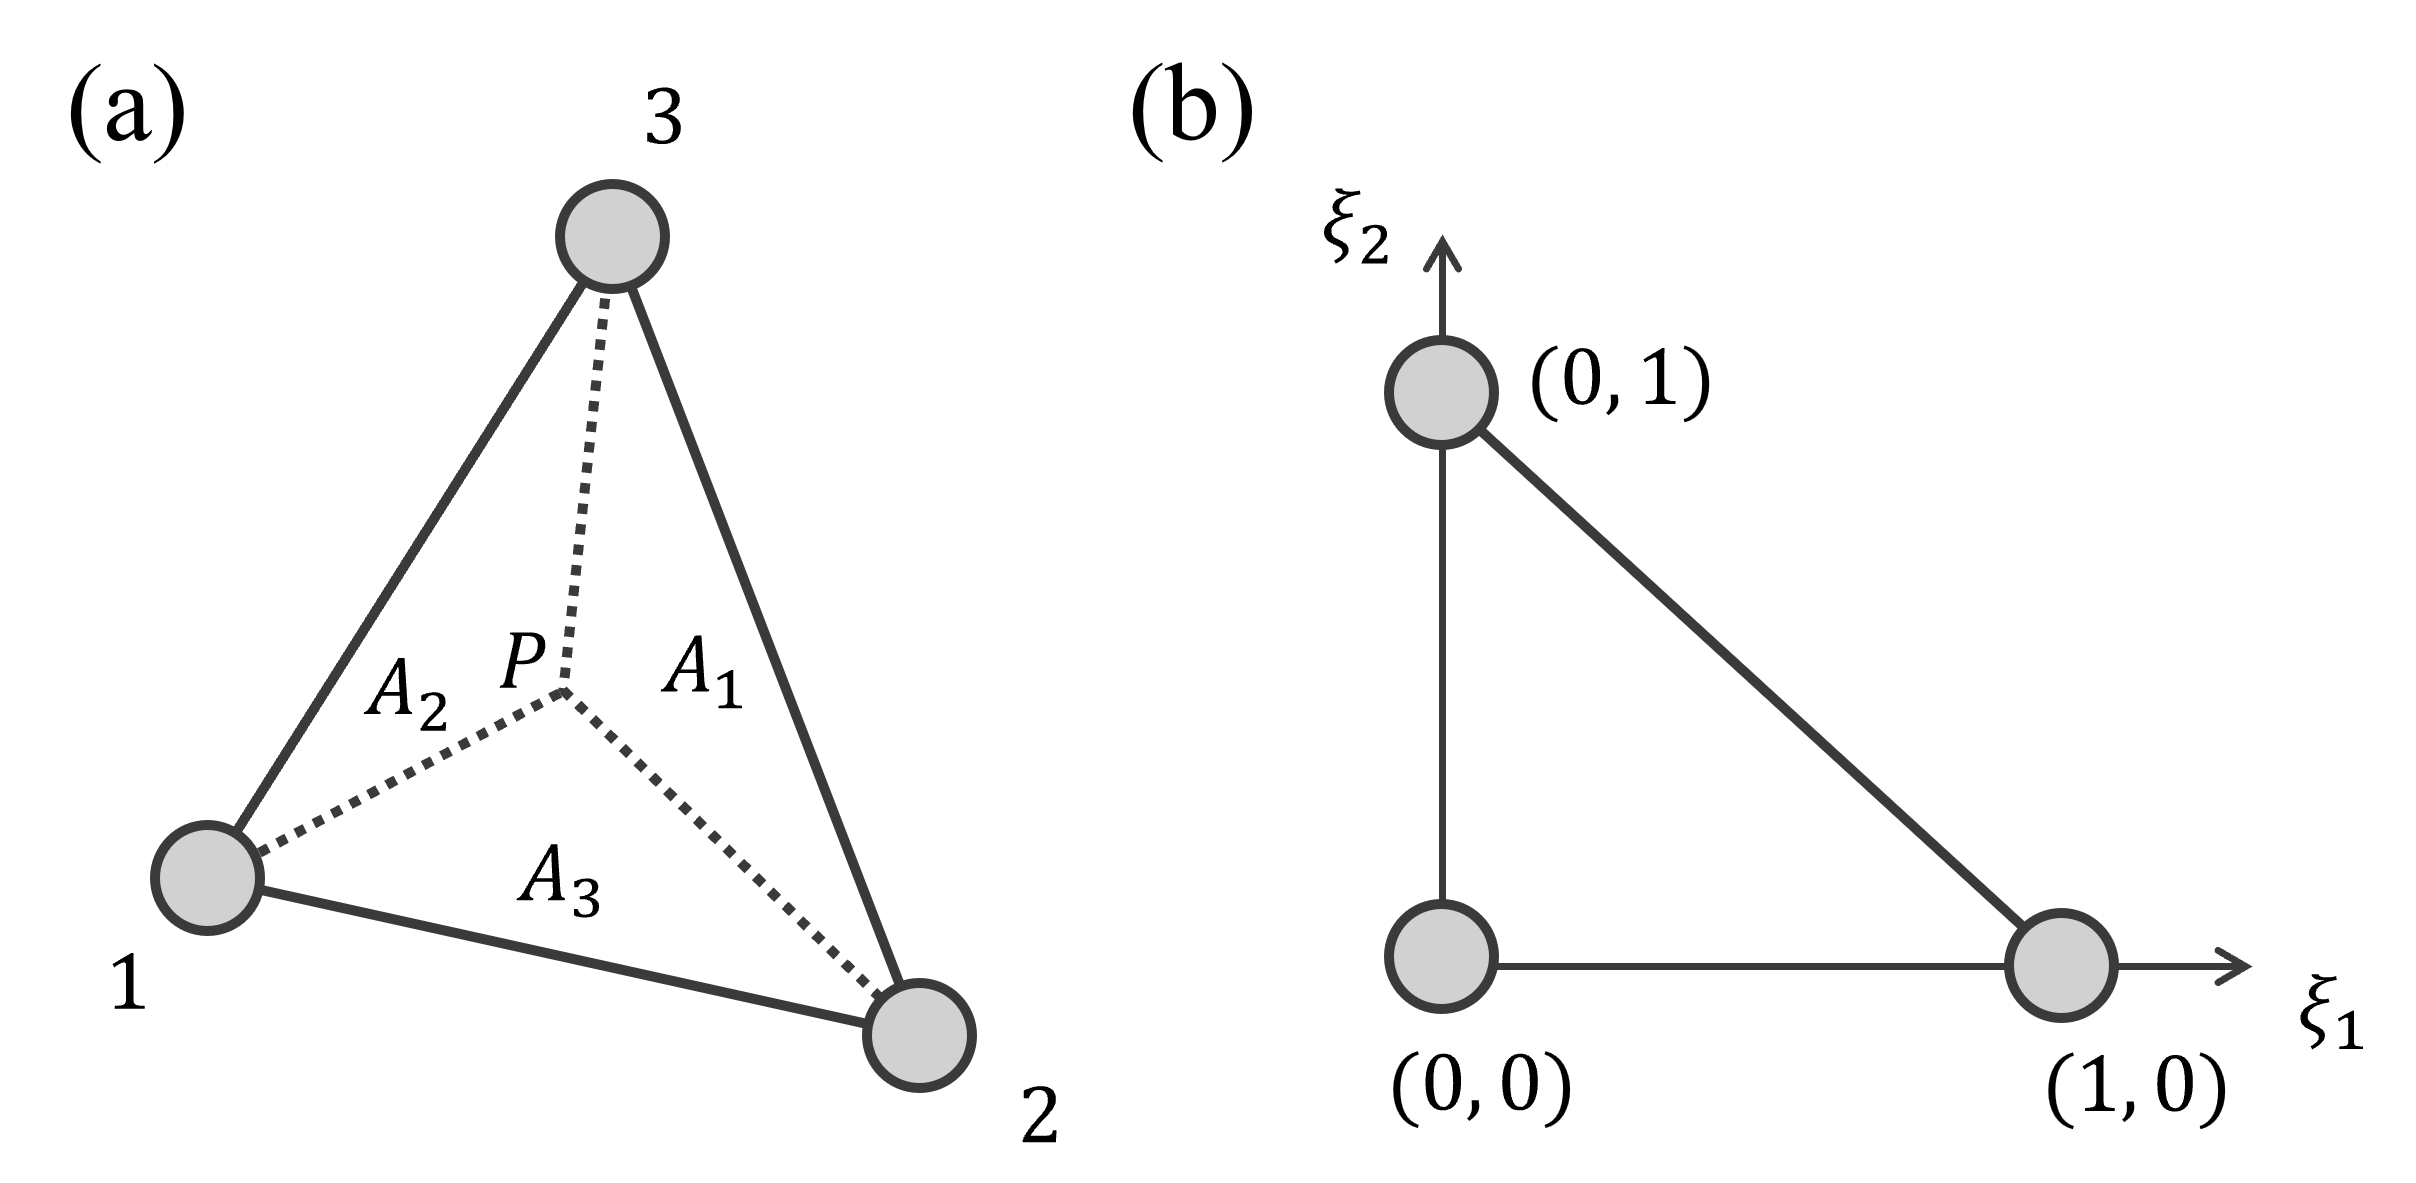
\includegraphics[width = 10cm]{fig1_6.png}
\caption{(a)面積座標(b)親座標と親領域}
\end{center}
\end{figure}

\subsection{2次元空間におけるガウス積分}
\subsubsection{三角形要素の場合}
2次元三角形領域に対するガウス積分は図1.6(b)の三角形領域$\Omega'$に対し定義されている。そのため、図1.6(a)もしくは図1.5のような物理領域$\Omega$に対する積分$I=\int_\Omega f(x, y)dxdy$を求めるためには、まずは変数変換をしなければならない。\par
$f(x, y)$から$f(\xi_1, \xi_2, \xi_3)$への変換は一般的に自明であろう。例えば式(1.21)の関係式より導出できる。ちなみにFEMに限って言えば、積分対象は$\theta^e$などであって、そもそも親領域での定義を用いているので、変換作業が不要だったりする。\par
微小領域の変換はヤコビ行列を用いて書き表すことができる。親座標と物理座標に式(1.20)の関係があるならば、ヤコビ行列は以下の通りである。
\begin{equation}
J^e=
\begin{bmatrix}
x^e_1 - x^e_3 & y^e_1 - y^e_3 \\
x^e_2 - x^e_3 & y^e_2 - y^e_3 \\
\end{bmatrix}
\end{equation}\par
以上より、所望の積分値は$I=\int_{\Omega'}|J^e|f(\xi_1, \xi_2, \xi_3){\rm d}\xi_1{\rm d}\xi_3{\rm d}\xi_3$と書き表すことができる。証明は省くが、この値は
\begin{equation}
I=\sum_{i=1}^3 W|J^e|f(\bm \xi_i)
\end{equation}
より求まる。ここで$W_i=0.1666666666$であり、
\begin{equation}
\begin{array}{l}
\bm \xi_1=(\xi_{11}, \xi_{12}, \xi_{13})=(0.1666666666, 0.1666666666, 1 - \xi_{11}-\xi_{12}) \\
\bm \xi_2=(\xi_{21}, \xi_{22}, \xi_{23})=(0.6666666666, 0.1666666666, 1 - \xi_{21}-\xi_{22}) \\
\bm \xi_3=(\xi_{31}, \xi_{32}, \xi_{33})=(0.1666666666, 0.6666666666, 1 - \xi_{31}-\xi_{32}) \\
\end{array}
\end{equation}
である(3節点以上の三角形要素におけるガウス積分など、より一般的な議論については他書参照)。

\subsubsection{四角形要素の場合}
2次元四角形要素におけるガウス積分も前項と同様である。積分領域には図1.4(a)の親領域を用いる。図1.4(b)のような物理領域を考えたとき、微小面積には$|J^e|{\rm d}\xi{\rm d}\eta={\rm d}x{\rm d}y$の関係がある。以上より所望の積分値は
\begin{equation}
I=\int_{-1}^1 {\rm d}\xi\int_{-1}^1{\rm d}\eta|J^e(\xi, \eta)|f(\xi, \eta) \notag
\end{equation}
と書き表せる。これは1次元におけるガウス積分を2回施すことにより求めることができる。つまり、表1.1の重みと積分点を用いて
\begin{equation}
I=\sum_{i=1}^2\sum_{j=1}^2W_iW_j|J^e(\xi_i, \eta_j)|f(\xi_i, \eta_j)
\end{equation}
より求めればよい。

\subsection{3次元空間における形状関数}
本章の最後に、3次元空間における形状関数について議論する。3事件空間における要素形状として有名なものに8節点六面体と4節点四面体があるが、これはそれぞれ四角形要素と三角形要素に類似する。したがって形状関数の導出も1.3節とほとんど同じである。

\subsubsection{8節点四面体要素}
\begin{figure}[t]
\begin{center}
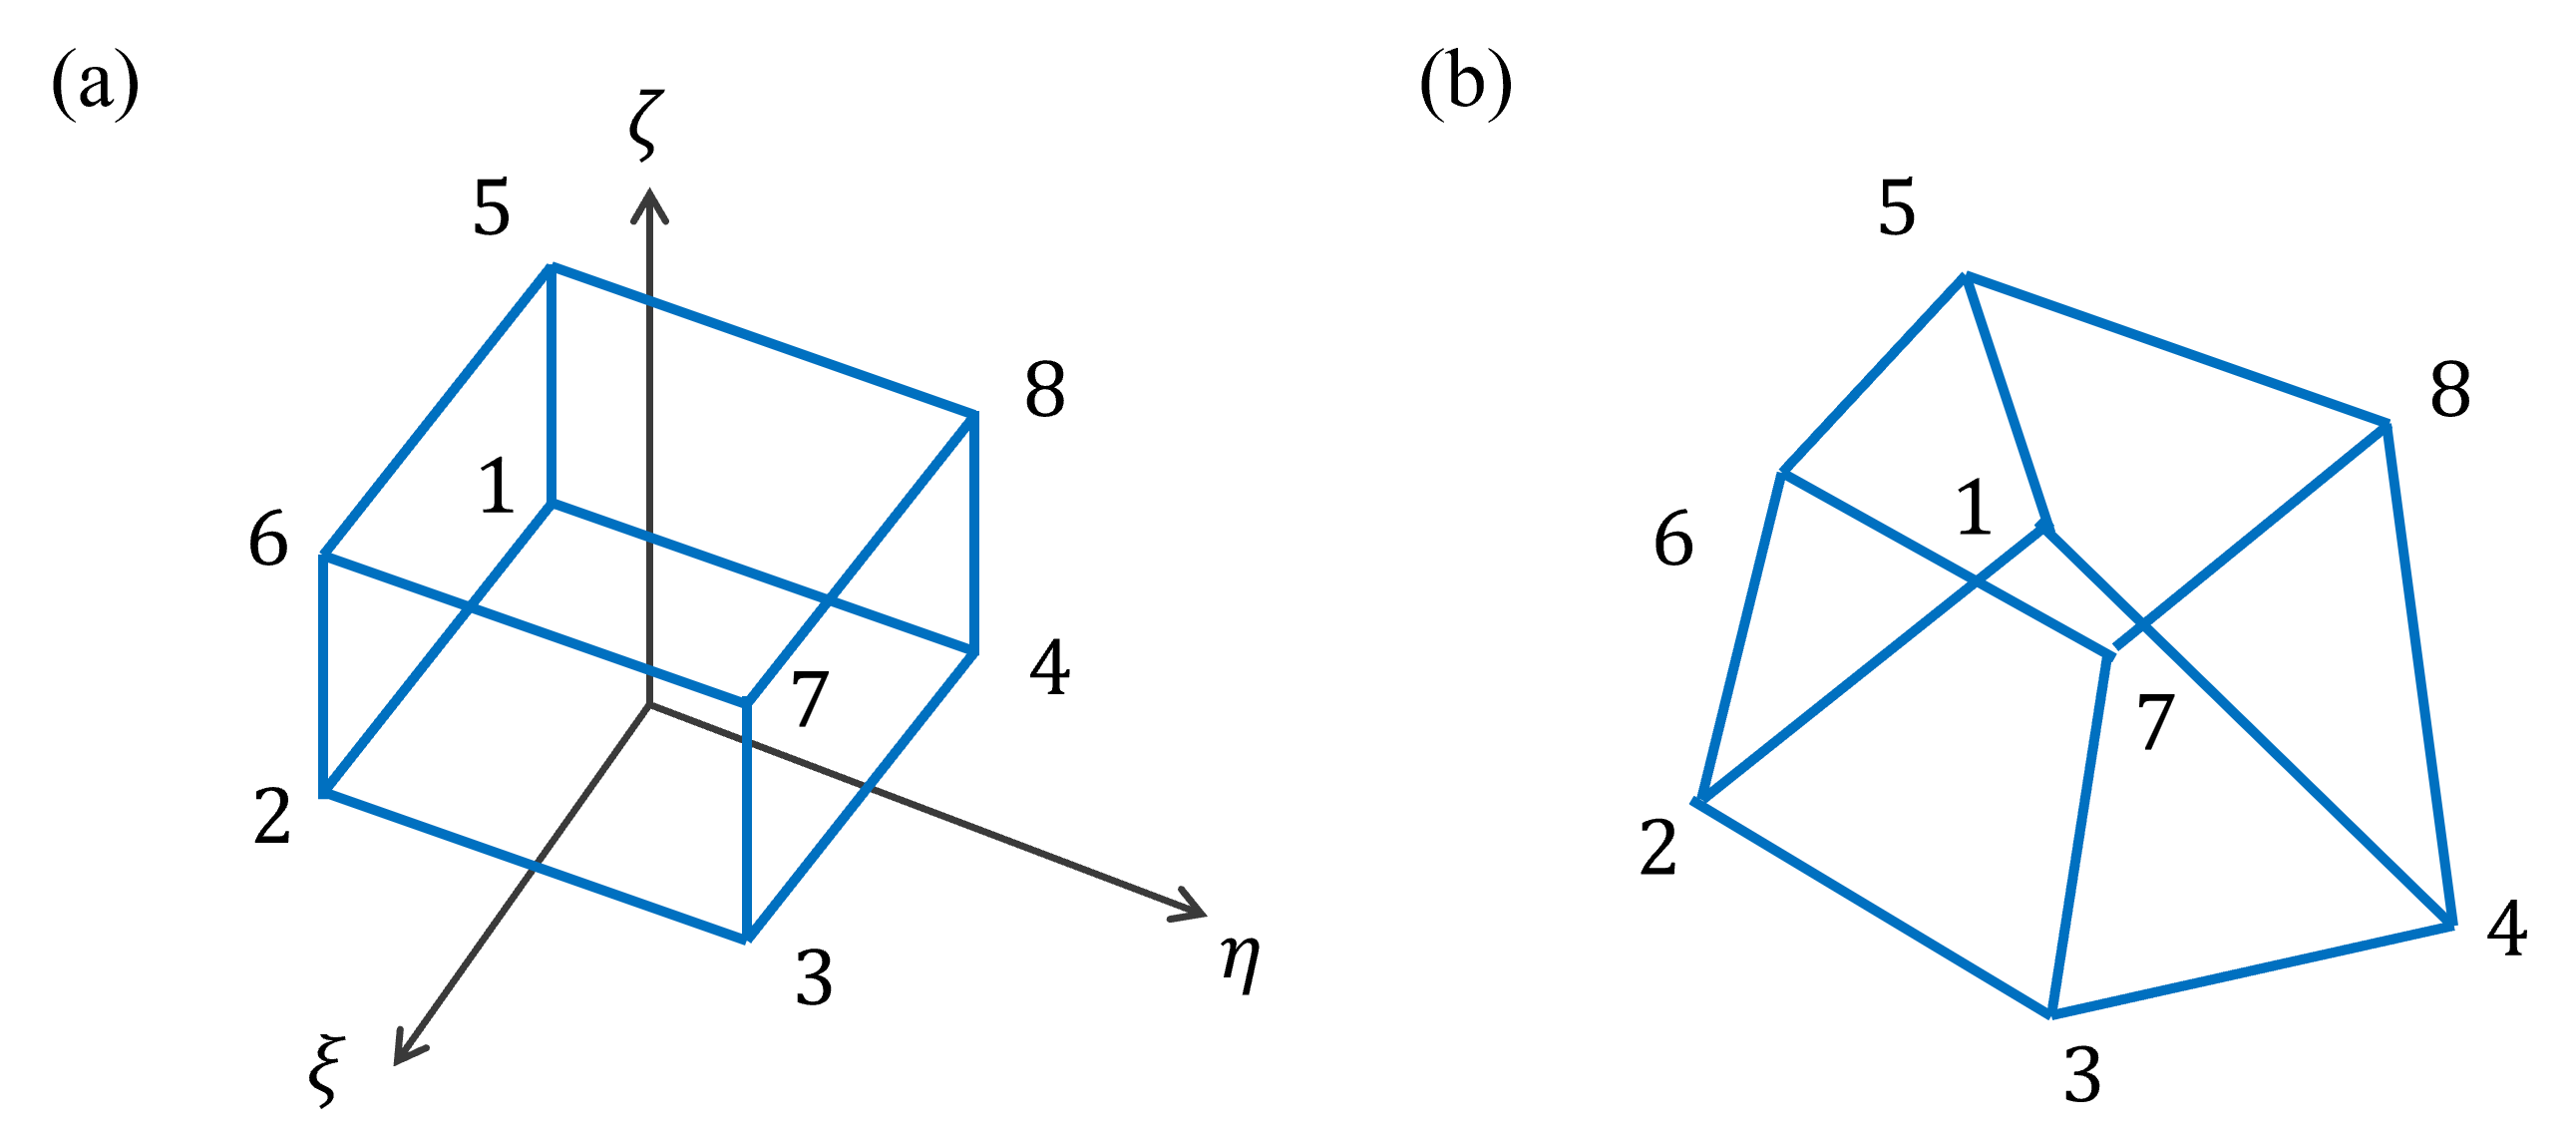
\includegraphics[width = 10cm]{fig1_7.png}
\caption{8節点六面体要素(a)親座標(b)物理座標}
\end{center}
\end{figure}
図1..7に8節点六面体要素の物理領域と親領域を示す。親領域は一辺の長さが2で中心が原点にある立方体で、図1.7(a)のように番号を割り振る。8節点であるため、形状関数も8つある訳だが、それぞれは式(1.3)の積で表すことができる。
\begin{equation}
N_i(\xi, \eta, \zeta)=N_j(\xi)N_k(\eta)N_l(\zeta)
\end{equation}
上式にある下付き添え字の組み合わせを表1.3に示す。\par

\begin{table}[t]
\begin{center}
\caption{式(1.27中下付き添え字の組み合わせ)}
\begin{tabular}{c|cccccccc}
\hline
i & 1 & 2 & 3 & 4 & 5 & 6 & 7 & 8 \\
j & 1 & 2 & 2 & 1 & 1 & 2 & 2 & 1 \\
k & 1 & 1 & 2 & 2 & 1 & 1 & 2 & 2 \\
l & 1 & 1 & 1 & 1 & 2 & 2 & 2 & 2 \\ \hline
\end{tabular}
\end{center}
\end{table}

式(1.27)に従う形状関数行列により、物理座標および物理量分布は以下の式で書き表される。
\begin{equation}
x = N\bm x^e,~~~y = N\bm y^e,~~~z = N\bm z^e,~~~\theta(\xi, \eta, \zeta) = N\bm \theta^e
\end{equation}
この形状関数行列のBマトリックスは式(1.16)のように書き表される。ただし3次元空間の場合は$G=(\partial_\xi, \partial_\eta, \partial_\zeta)^{\rm T}$であり、ヤコビ行列は
\begin{equation}
J^e=
\begin{bmatrix}
\partial_\xi x & \partial_\xi y & \partial_\xi z \\
\partial_\eta x & \partial_\eta y & \partial_\eta z \\
\partial_\zeta x & \partial_\zeta y & \partial_\zeta z \\
\end{bmatrix} \notag
\end{equation}
となる。

\subsubsection{4節点四面体要素}
\begin{figure}[b]
\begin{center}
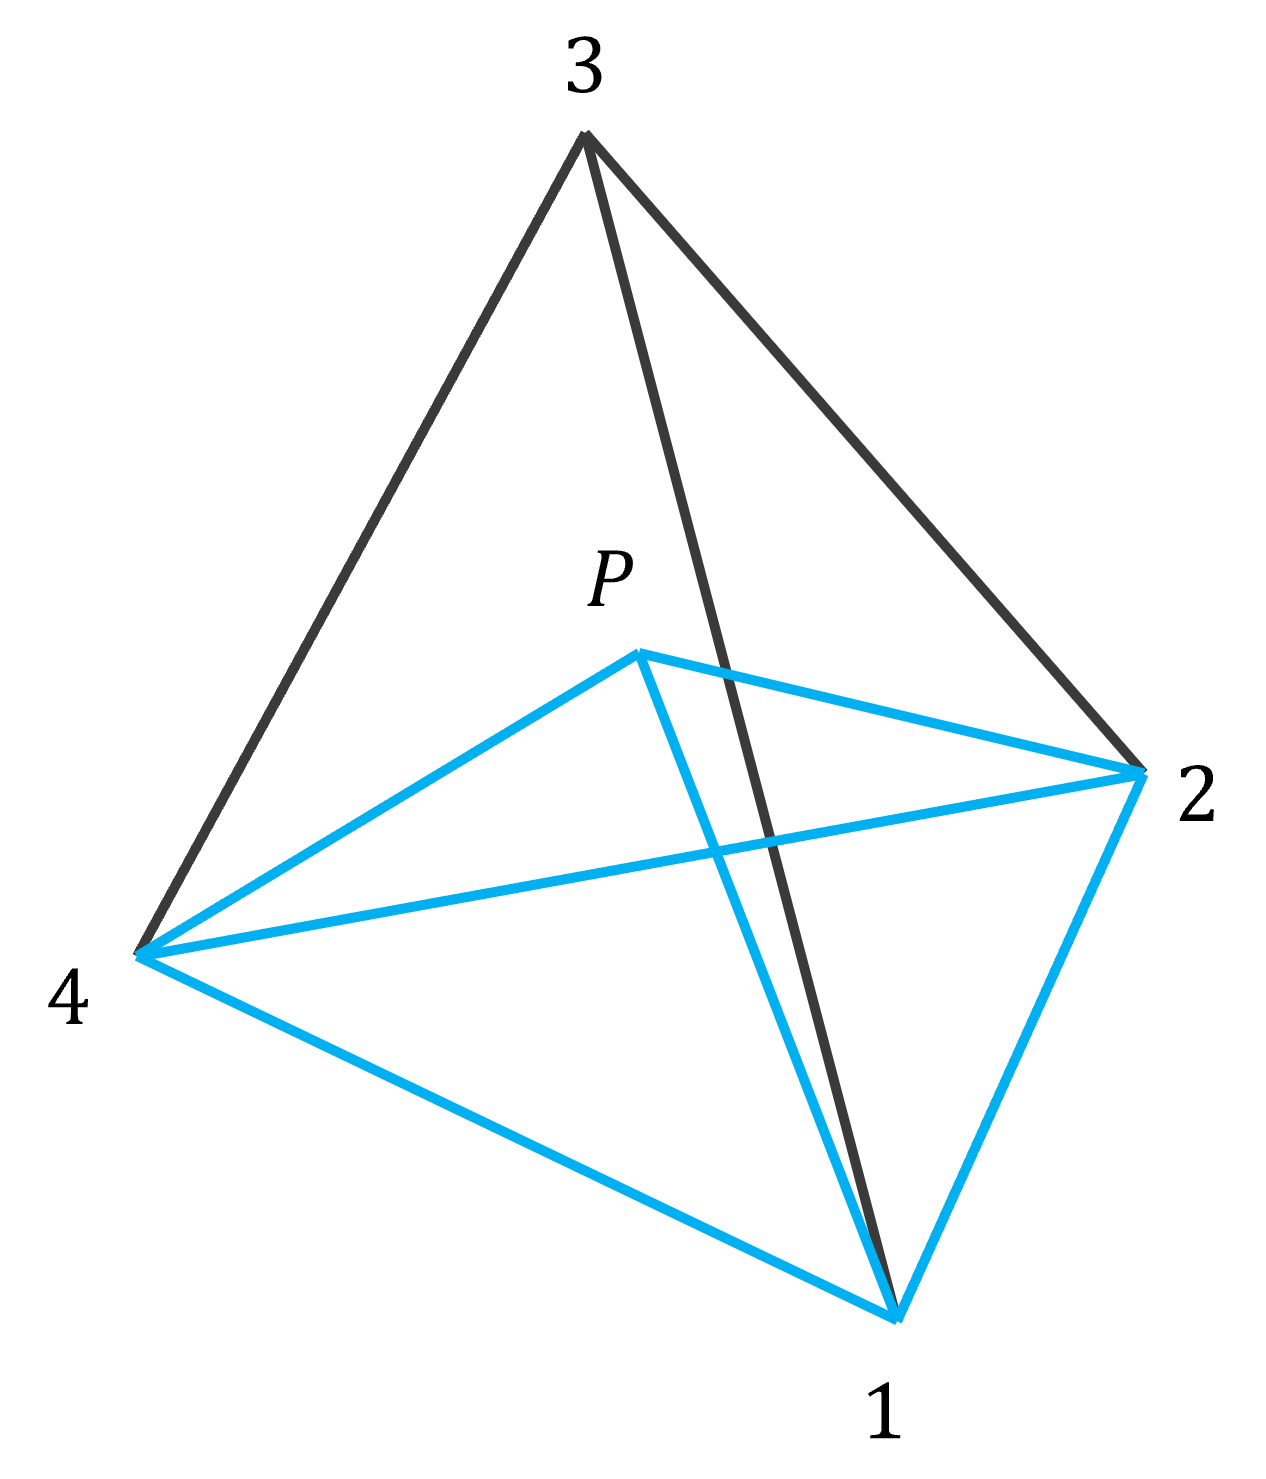
\includegraphics[width = 4cm]{fig1_8.png}
\caption{4節点四面体要素の体積座標}
\end{center}
\end{figure}

4節点四面体要素では面積座標ではなく体積座標$(\xi_1, \xi_2, \xi_3, \xi_4)$を考える。例えば$\xi_3$は(四面体124Pの体積)/(四面体1234の体積)であり、他の座標値についても同様に定義されている。物理座標と体積座標は一対一に対応しており、
\begin{equation}
\begin{bmatrix}
1 & x & y & z
\end{bmatrix}=
\begin{bmatrix}
1 & 1 & 1 & 1 \\
x^e_1 & x^e_2 & x^e_3 & x^e_4 \\
y^e_1 & y^e_2 & y^e_3 & y^e_4 \\
z^e_1 & z^e_2 & z^e_3 & z^e_4 \\
\end{bmatrix}
\begin{bmatrix}
\xi_1 \\ \xi_2 \\ \xi_3 \\ \xi_4
\end{bmatrix} \notag
\end{equation}
の関係がある。また、1.3.3項と同様に物理量は
\begin{equation}
\theta(\xi_1, \xi_2, \xi_3, \xi_4)=\sum \theta^e_i \xi_i
\end{equation}
で書き表わされる。

\subsection{3次元空間におけるガウス積分}
1.5節の議論が1.3節と同様であったように、本節の内容も1.4節と同様である。
\subsubsection{四面体要素の場合}
所望の積分値$I=\int_{\Omega}f(x, y, z){\rm d}x{\rm d}y{\rm d}z$は
\begin{equation}
I=\sum_{i=1}^4 W|J^e|f(\bm \xi_i)
\end{equation}
となる。ここで$W=0.25$であり、1.5.2項の形状関数を用いたならばヤコビ行列は
\begin{equation}
J^e=
\begin{bmatrix}
x^e_1 - x^e_4 & y^e_1 - y^e_4 & z^e_1 - z^e_4 \\
x^e_2 - x^e_4 & y^e_2 - y^e_4 & z^e_2 - z^e_4 \\
x^e_3 - x^e_4 & y^e_3 - y^e_4 & z^e_3 - z^e_4 \\
\end{bmatrix} \notag
\end{equation}
である。また、積分点は
\begin{equation}
\begin{array}{l}
\bm \xi_1 = (\xi_{11}, \xi_{12}, \xi_{13}, \xi_{14})=(0.58541020, 0.13819660, 0.13819660, 1 - \xi_{11}-\xi_{12}-\xi_{13}) \\
\bm \xi_2 = (\xi_{21}, \xi_{22}, \xi_{23}, \xi_{24})=(0.13819660, 0.58541020, 0.13819660, 1 - \xi_{21}-\xi_{22}-\xi_{23}) \\
\bm \xi_3 = (\xi_{31}, \xi_{32}, \xi_{33}, \xi_{34})=(0.13819660, 0.13819660, 0.58541020, 1 - \xi_{31}-\xi_{32}-\xi_{33}) \\
\bm \xi_4 = (\xi_{41}, \xi_{42}, \xi_{43}, \xi_{44})=(0.13819660, 0.13819660, 0.13819660, 1 - \xi_{41}-\xi_{42}-\xi_{43}) \\
\end{array}
\end{equation}
である(より一般的な議論は他書を参照)。

\subsubsection{八面体要素の場合}
1.4.2項と同様に、1次元におけるガウス積分を3解施す。従って積分値は
\begin{equation}
I=\int_\Omega f(x, y, z){\rm d}x{\rm d}y{\rm d}z=\int_{-1}^1{\rm d}\xi\int_{-1}^1{\rm d}\eta\int_{-1}^1{\rm d}\zeta f(\xi, \eta, \zeta)|J^e(\xi, \eta, \zeta)|=\sum_{i=1}^2\sum_{j=1}^2\sum_{k=1}^2W_iW_jW_k|J^e(\xi_i, \eta_j, \zeta_k)|f(\xi_i, \eta_j, \zeta_k)
\end{equation}
となる。

\section{定常スカラー場問題における有限要素法}
本章では最も理解が容易と思われる定常スカラー場問題のFEMについて議論する。題材には異方性がある熱伝導方程式
\begin{equation}
\bnabla \cdot (K\bnabla T)+b=0~(\bm r \in V),~~~K\bnabla T(\bm r)\cdot \bm n =q(\bm r)~(\bm r \in F_t),~~~T(\bm r)=T_0(\bm r)~(\bm r \in F_u)
\end{equation}
を用いることにしよう。ここで$K$は熱伝導率の2階テンソル、$T$は温度、$b$はソースである。また、$F_t$はノイマンB.C.が与えられている位置の集合であり、$F_u$はディリクレB.C.が与えられている位置の集合である。式(2.1)ような我々がよく目にする支配方程式のことを強形式と言う。FDMではこれを直接離散化するのに対し、FEMでは特別な処理を施し、弱形式と呼ばれる形に変換する。

\subsection{弱形式}
物理現象が式(2.1)を満たすならば、任意の関数$w$に対して
\begin{equation}
\int_V w\left\{\bnabla \cdot (K\bnabla T)+b\right\}{\rm d}\bm r=0,~~~\int_{F_t}w(K\bnabla T \cdot \bm n - q)=0
\end{equation}
が成立するはずである。この任意の関数$w$のことを重み関数と言い、式(2.2)のことを弱形式と言う。\par
式(2.2)が任意の$w$で成立するならば、強形式と弱形式は同値であることが判っている。そして先述の通り、FEMはこの弱形式から近似関数$T(\bm r)$を導出する。式(2.2)を満たす関数の集合を候補解、ならびに候補解の各元を試行関数と言う。FEMでは候補解のうちディリクレB.C.を満たす関数に絞って解を求める。なお、式(2.2)にはディリクレB.C.の情報が含まれていないが、今のところ問題はない。弱形式を求めて離散化した後、その離散式にディリクレB.C.の制約も付与する。例えばFDMではディリクレB.C.の制約をソース項に反映させるか、連立一次方程式に明示的に$T(\bm r)=T_0(\bm r)$なる方程式を追加するであろう。FEMでも同様な処理を施すので、今は考えなくても済むわけである(逆に今の段階で支配方程式とノイマンB.C.の両方を考えることはFDMと異なり、特徴的な点と言える)。\par
さて、式(2.1)より$b \neq 0$の場合、$T$の2回微分も非ゼロでなければならないことが分かる。これは関数$T$が$C^2$級関数であることを意味している。もちろん物理的には正しいが、この要求は数値計算的に見て厳しい。例えばいくつかの節点で領域を分割し、各部分領域で線形近似したような関数$T$は$C^2$級関数の条件を満たさない。しかしながら線形近似は数値計算でよく用いるものであるため、熱伝導方程式でも使いたくなったりするだろう(この議論は2回微分を有する支配方程式全般に言える)。そこで、以下ののグリーンの公式を考える。
\begin{equation}
\int_V w\bnabla \cdot \bm f {\rm d}\bm r=\int_Fw\bm f \cdot \bm n{\rm d}\bm r - \int_V \bnabla w\cdot \bm f{\rm d}\bm r \notag
\end{equation}
グリーンの公式中の$\bm f$を$K\bnabla T$に書き換え、式(2.2)の一つ目の式に代入すると、
\begin{equation}
\int_V w\left\{\bnabla \cdot (K\bnabla T)+b\right\}{\rm d}\bm r=\int_{F_t}w(K\bnabla T)\cdot \bm nd \bm r + \int_{F_u}w(K\bnabla T)\cdot \bm n{\rm d} \bm r - \int_V\bnabla w \cdot (K\bnabla T) {\rm d} \bm r+\int_Vwb{\rm d}\bm r=0 \notag
\end{equation}
を得る(ここで境界における積分を右辺第一項と二項のように分割した)。\par
次に、関数$w$についてディリクレB.C.上の$\bm r$ではゼロ、つまり$w(\bm r)=0~(\bm r \in F_u)$であるとする。この条件は重み関数の任意性を損なうことになるが、強形式と弱形式の同値性は損なわれない(詳細な説明は他書に譲るが、こう設定することで連立一次方程式の求解が容易になる)。このとき、上式は
\begin{equation}
\int_V\bnabla w \cdot (K\bnabla T) {\rm d} \bm r = 
\int_{F_t}w(K\bnabla T)\cdot \bm n{\rm d} \bm r + \int_Vwb{\rm d}\bm r
\end{equation}
と書き直される。右辺第一項について、ノイマンB.C.より$K\bnabla T\cdot \bm n$の値は既知であるため、最終的に以下の弱形式を得る。
\begin{equation}
\int_V\bnabla w \cdot (K\bnabla T) {\rm d} \bm r = 
\int_{F_t}wq{\rm d} \bm r + \int_Vwb{\rm d}\bm r \notag
\end{equation}
以上より、$T$に関する条件が$C^1$級関数まで緩めることができた。ここまでの導出結果を以下に纏める。
\begin{tcolorbox}[title=定常熱伝導問題における弱形式]
以下の熱伝導方程式を考える。
\begin{equation}
\bnabla \cdot (K\bnabla T)+b=0~(\bm r \in V),~~~K\bnabla T(\bm r)\cdot \bm n =q(\bm r)~(\bm r \in F_t),~~~T(\bm r)=T_0(\bm r)~(\bm r \in F_u)
\end{equation}
ここで$K$は熱伝導率の2階テンソル、$T$は温度、$b$はソースである。また、$F_t$はノイマンB.C.が与えられている位置の集合であり、$F_u$はディリクレB.C.が与えられている位置の集合である。重み関数$w$について$w(\bm r)=0~(\bm r \in F_u)$としたとき、弱形式は以下のように表される。
\begin{equation}
\int_V\bnabla w \cdot (K\bnabla T) {\rm d} \bm r = 
\int_{F_t}wq{\rm d} \bm r + \int_Vwb{\rm d}\bm r
\end{equation}
\end{tcolorbox}

\subsubsection{ロビン境界条件が存在する場合の弱形式}
本項ではロビンB.C.
\begin{equation}
A(\bnabla T \cdot \bm n) + BT=C \notag
\end{equation}
がある場合を考える。なお、ロビンB.C.は$A=0$のときディリクレB.C.と、$B=0$のときノイマンB.C.と同一視できるので、本項で扱う問題では全ての境界面がロビンB.C.で書き表されるとする。従って、このときの強形式は
\begin{equation}
\bnabla \cdot (K\bnabla T)+b=0~(\bm r \in V),~~~A(\bnabla T \cdot \bm n) + BT=C~(\bm r \in F)
\end{equation}
のように書き表される。\par
ロビンB.C.に変わったとしても、弱形式の導出は前回と同様である。境界$F$のうち、$A=0$となる部分集合、つまりディリクレB.C.である部分集合を$F_u$とし、それ以外を$F_t$とする。同様の手順で計算を進めれば式(2.3)が得られる訳だが、$\bm r \in F_t$において$(K\bnabla T)\cdot \bm n=(C-BT)/A$であるため、これを代入すると
\begin{equation}
\int_V\bnabla w \cdot (K\bnabla T) {\rm d} \bm r = 
\int_{F_t}w\frac{C-BT}{A}{\rm d} \bm r + \int_Vwb{\rm d}\bm r
\end{equation}
を得る。以上がロビンB.C.における弱形式である。


\subsection{離散化とアセンブリ}
後述するように、FEM解析は最終的に連立一次方程式に帰着する。解であるベクトルの各項は各節点における物理量である。この連立一次方程式は各要素に対してではなく解析領域全体に対して与えられる。\par
前節より得た支配方程式の弱形式は離散化された状態ではなく、節点という考え方もしていない。そこで、まずは計算機で解析可能な形にするために、解析領域を節点と要素により離散化する。そして各要素における物理量の分布を多項式で近似し、その近似関数が弱形式を満たすように近似関数の係数を決めていく。\par
この一連の処理には離散化とアセンブリという処理が含まれている。離散化とは式(2.5)などにある分布関数を近似関数に変えたのち、計算しやすい形に変換していく処理である。他方のアセンブリとは離散化より得た式から連立一次方程式を得る処理のことを指す。

\subsubsection{離散化}
本項では式(2.5)の離散化について議論していく。この場合、求めるべきものは関数$T$である。そこで解析領域を要素で分割し、要素$e$毎に補間関数$T^e(\bm r)$を設定する。前章の通り、補間関数は$e$の形状関数行列$N^e(\bm r) \in \mathbb{R}^{1 \times n_n}$を用いて
\begin{equation}
T^e(\bm r)=N^e(\bm r)\bm T^e
\end{equation}
と書き表される。ここで$n_n$は要素$e$の節点数である。また$\bm T^e$は$\bm T^e=(T^e_1, ..., T^e_{n_n})^{\rm T}$であり、各節点の物理量を纏めたベクトルである。\par
離散化での狙いは、関数$T$を多項式で補間し、式(2.5)の積分計算をガウス積分で済ませることである。しかしながら関数$w$が存在するゆえに、今の段階でそれはできない。そこで$w$に関しても多項式で近似することを考える。関数$w$も連続でなければならないので、$T$と同じ形状関数行列を用いて
\begin{equation}
w^e(\bm r)=N^e(\bm r)\bm w^e
\end{equation}
のように近似できる。ここで$w^e(\bm r)$は要素$e$における重み関数、$\bm w^e$は節点上における重み関数値である。以上より、式(2.8)(2.9)を式(2.5)に代入すると、以下の式を得る。
\begin{equation}
\sum_e\left\{ \int_{V_e}B^e\bm w^e\cdot(KB^e\bm T^e){\rm d}\bm r - \int_{F_{te}}N^e\bm w^eq{\rm d}\bm r-\int_{V_e}N^e\bm w^eb{\rm d}\bm r  \right\}=0 \notag
\end{equation}
ここで$V_e$は各要素の領域、$F_{te}$は各要素においてノイマンB.C(もしくはロビンB.C.).が定義されている領域(空集合もあり得る)である。上式のうち$\bm w^e$と$\bm T^e$は$\bm r$に依存しないので、
\begin{equation}
\sum_e\bm w^e \cdot \left\{ \left( \int_{V_e} B^{e\rm T}KB^e {\rm d}\bm r \right)\bm T^e-\int_{F_{te}}qN^{e\rm T}{\rm d}\bm r-\int_{V_e}bN^{e\rm T}{\rm d}\bm r \right\}=0 \notag
\end{equation}
のように書き換えることができる。
上式のうち
\begin{equation}
K^e = \int_{V_e} B^{e\rm T}KB^e {\rm d}\bm r \in \mathbb{R}^{n_n \times n_n}
\end{equation}
のことを要素係数行列という。ここで$n_n$は要素$e$に含まれる節点の数である。また、
\begin{equation}
\bm f^e = \int_{F_{te}}qN^{e\rm T}{\rm d}\bm r+\int_{V_e}bN^{e\rm T}{\rm d}\bm r \in \mathbb{R}^{1\times n_n}
\end{equation}
のことを要素ソース行列と言う。式(2.10)(2.11)はガウス積分で求めればよい。以上より上式は
\begin{equation}
\sum_e \bm w^e\cdot(K^e\bm T^e-\bm f^e)=0
\end{equation}
のように書くことができる。以上が離散化処理である。

\subsubsection{アセンブリ処理}
離散化により式(2.5)から式(2.12)を得たが、まだ数値計算できる状態にはない。全ての要素$e$に対して$\bm w^e$には任意性があるためである。そこでアセンブリ処理を考える。\par
アセンブリ処理とは式(2.12)から全節点における物理量に関する連立一次方程式を導出する処理である。まず、全節点における$T$の値を纏めたベクトル$\bm T \in \mathbb{R}^n$を考える。ここで$n$は解析領域内にある節点の数である。同様に節点上の重み関数値を纏めたベクトルを$\bm w \in \mathbb{R}^n$とする。\par
次に$\bm T$から$\bm T^e$を抽出するオペレータ、つまり$L^e\bm T = \bm T^e$を満たす行列を要素毎に定義する。この$L^e$は当然ながら$L^e\bm w=\bm w^e$も満たす。すると式(2.12)は
\begin{equation}
\sum_e (L^e\bm w) \cdot (K^eL^e\bm T - \bm f^e) = 0 \notag
\end{equation}
のように書き換えることができる。$\bm w$は要素$e$の総和の外に出すことができるため、上式は
\begin{equation}
\bm w \cdot (K\bm T - \bm f),~~~K=\sum_eL^{e\rm T}K^eL^e,~~~\bm f=\sum_eL^{e\rm T}\bm f^e \notag
\end{equation}
と更に書き換えることができる。ここで$K \in \mathbb{R}^{n \times n}$のことを全体係数行列、$\bm f \in \mathbb{R}^n$のことを全体ソース行列と言う。\par
弱形式(2.5)はディリクレB.C.の領域でゼロとなる任意の関数$w$で成立しなければならなかったが、離散化した今となってはディリクレB.C.上の節点に対する要素がゼロの任意のベクトル$\bm w$で成立しなければならないと言い換えられる。従って$K\bm T - \bm f = \bm r$と置いたとき$\bm w \cdot \bm r=\sum w_i r_i$であるため、明らかにディリクレB.C.上の節点以外では$r_i=0$とならなければならない。\par
一方でディリクレB.C.上の節点の$T$の値は所与である。したがってディリクレB.C.上の節点$i$に対して$K_{ij}=\delta_{ij}$および$f_i=T_i$と書き換えれば、連立一次方程式$K\bm T=\bm f$より所望の分布$\bm T$が得られることになる。

\subsubsection{全体係数行列および全体ソース行列の効率的な求め方}
前項より$K$および$\bm f$が得られれば、あとは連立一次方程式の求解で所望の分布$\bm T$が求まることが分かった。$K$や$\bm f$を得るには行列$L^e$が必要になるが、実はプログラミングスクリプト上で$L^e$を明示的に定義することは稀である。$L^e$は唯々要素を抽出しているだけなので、要素係数行列(もしくは要素ソース行列)の値を全体係数行列(もしくは全体ソース行列)の適当な要素に足せば済む話であろう。\par
例えば要素$e$において$i$番目の節点が、全体のベクトルの$j$番目に対応している場合、つまり$T^e_i$と$T_j$が対応している場合を考える。いま$\bm f^e$はガウス積分より求まるのであった。$\bm f$については$f^e_i$の値を$f_j$に足せばよい。全体係数行列についても同様である。要素$e$の$p$番目の節点が、全体のベクトルの$q$番目に対応している場合、$K_{jq}$に$K_{ip}$の値を足せばよい。$K$および$\bm f$をゼロ行列とゼロベクトルで始め、全ての要素について足し合わせ処理を施せば、所望の$K$と$\bm f$が得られる。

\end{document}










